\documentclass[Alon2,singlecolor,11pt]{Alon}%
\usepackage{fixltx2e,fix-cm}
\usepackage[english]{babel}
\usepackage{epigrafica}
\usepackage[LGR,OT1]{fontenc}
%\usepackage{mathptmx,txfonts}
\usepackage{lmodern}
\usepackage{amssymb}
\usepackage{amsmath}
\usepackage{graphicx}
\usepackage{subcaption}
\usepackage{makeidx}
\usepackage{multicol}

\renewcommand{\sfdefault}{txss}

\usepackage{changepage}% for text width to include margin

\usepackage[breakable,skins]{tcolorbox}
\usepackage{customenvironments}

\frenchspacing
\tolerance=5000

\makeindex

\include{frontmatter/preamble}%place custom commands and macros here
\usepackage{version}
%\usepackage[breaklinks]{hyperref}



\title{Python for Mathematics}
\author{Vincent Knight}

\begin{document}

\frontmatter

%%%\maketitle%This is a placeholder titlepage, it will not be final.

%%%Placeholder for front matter


\title{Python for Mathematics} %This is a placeholder titlepage, it will not be final.
%%
\edition{First Edition}

\author{Vincent Knight}%%Used for authored book


\maketitle

\cleardoublepage
\thispagestyle{empty}
\vspace*{\stretch{1}}
\begin{center}
\Large\itshape
To Riggins.
\end{center}
\vspace{\stretch{2}}

\cleardoublepage
\setcounter{page}{7} %previous pages reserved for frontmatter to be added later
\tableofcontents
%%\listoffigures
%%\listoftables
\chapter*{Author Bios}

Ed/Author bios here


Aboritiorior maio. Optaess inullore cum autate niate nonem ut ario. Ut labor soloreped magniae ipsum etur sunt magnatiorpos nonsequi ut aliquideles quam quisque magnatia voluptae poreperiat.
Ibus, num escilla boreribus, utem qui arum fugitae rrorit que ide volum debit faci conseque nus as quo doluptatur autem qui odis dero esequis nihillaborio di audit ut moluptate opta dolorere vellabore verum fugita del molori occus pores est et fugiati audis enimus sitentur?
Possequ asperupita sedit, int.
Im dolo vid quo te quis dollam re ne que sime parchit aspici unto te accusam eium eium reptas sitatio etur?




\mainmatter

\part{Overview}
\documentclass{standalone}
\usepackage{tikz}


\begin{document}
        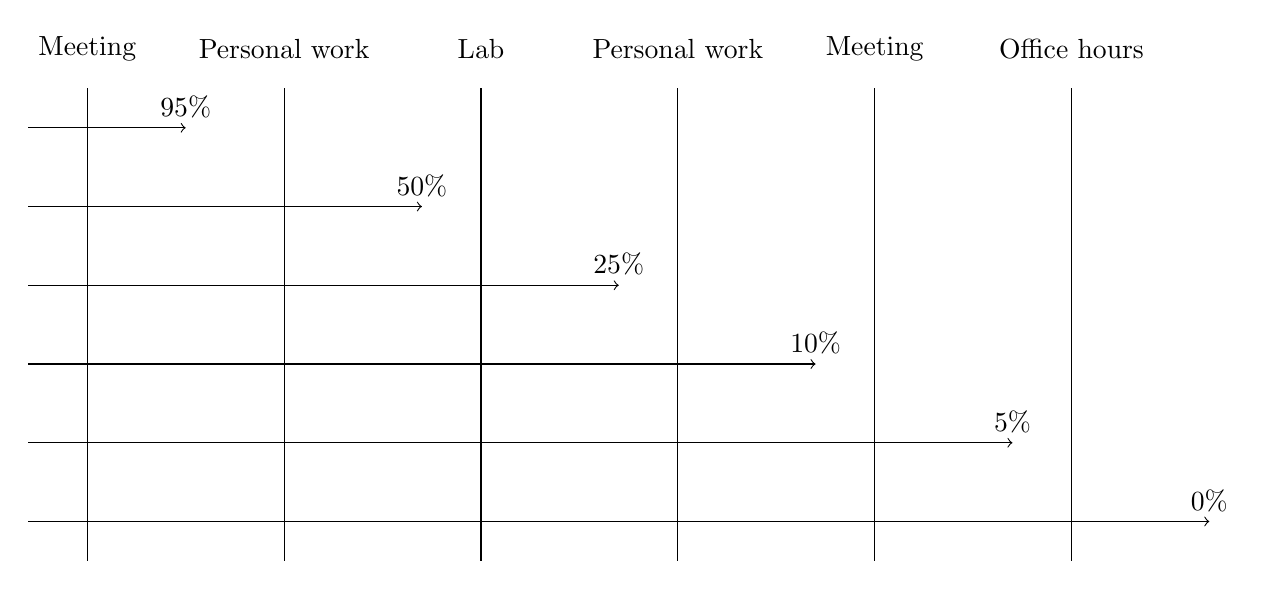
\begin{tikzpicture}
            \foreach \i/\label in {2.5/Meeting,
                                   5/Personal work,
                                   7.5/Lab,
                                   10/Personal work,
                                   12.5/Meeting,
                                   15/Office hours}
                {
                    \draw (\i, -5) -- (\i, 1);
                    \node at (\i, 1.5) {\label};
                }

            \draw [->] (1.75, .5) -- node [above, at end] {95\%} (3.75, .5);
            \draw [->] (1.75, -.5) -- node [above, at end] {50\%} (6.75, -.5);
            \draw [->] (1.75, -1.5) -- node [above, at end] {25\%} (9.25, -1.5);
            \draw [->] (1.75, -2.5) -- node [above, at end] {10\%} (11.75, -2.5);
            \draw [->] (1.75, -3.5) -- node [above, at end] {5\%} (14.25, -3.5);
            \draw [->] (1.75, -4.5) -- node [above, at end] {0\%} (16.75, -4.5);
    \end{tikzpicture}
\end{document}


\part{Tools for Mathematics}

\documentclass{standalone}
\usepackage{tikz}


\begin{document}
        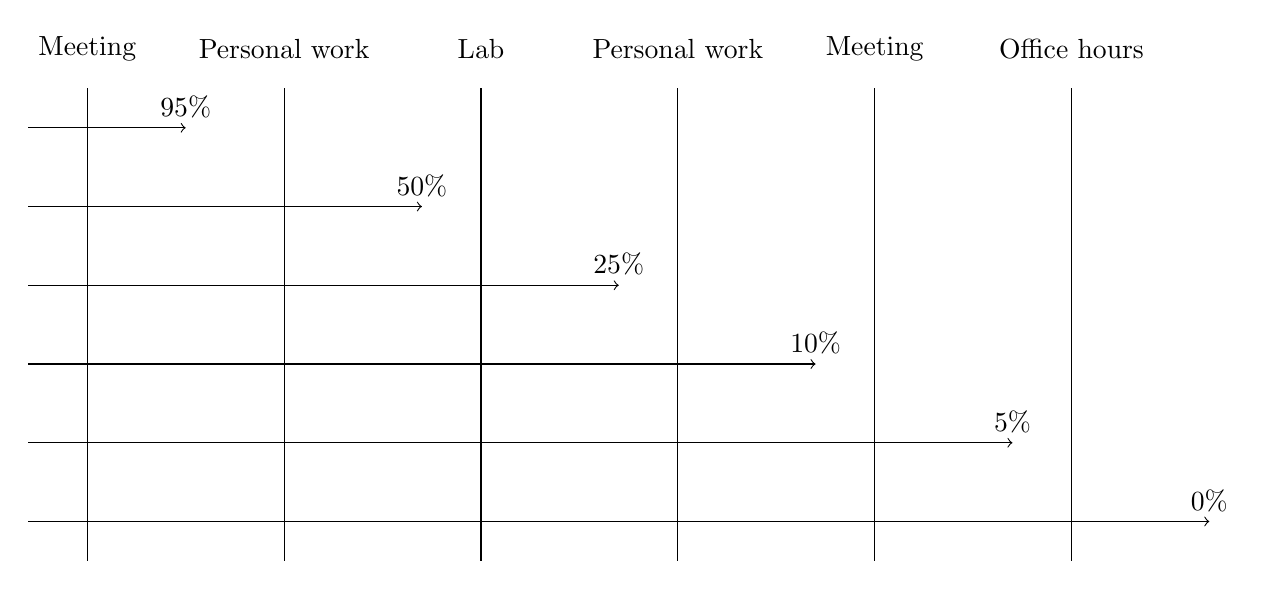
\begin{tikzpicture}
            \foreach \i/\label in {2.5/Meeting,
                                   5/Personal work,
                                   7.5/Lab,
                                   10/Personal work,
                                   12.5/Meeting,
                                   15/Office hours}
                {
                    \draw (\i, -5) -- (\i, 1);
                    \node at (\i, 1.5) {\label};
                }

            \draw [->] (1.75, .5) -- node [above, at end] {95\%} (3.75, .5);
            \draw [->] (1.75, -.5) -- node [above, at end] {50\%} (6.75, -.5);
            \draw [->] (1.75, -1.5) -- node [above, at end] {25\%} (9.25, -1.5);
            \draw [->] (1.75, -2.5) -- node [above, at end] {10\%} (11.75, -2.5);
            \draw [->] (1.75, -3.5) -- node [above, at end] {5\%} (14.25, -3.5);
            \draw [->] (1.75, -4.5) -- node [above, at end] {0\%} (16.75, -4.5);
    \end{tikzpicture}
\end{document}


\part{Building Tools}

\documentclass{standalone}
\usepackage{tikz}


\begin{document}
        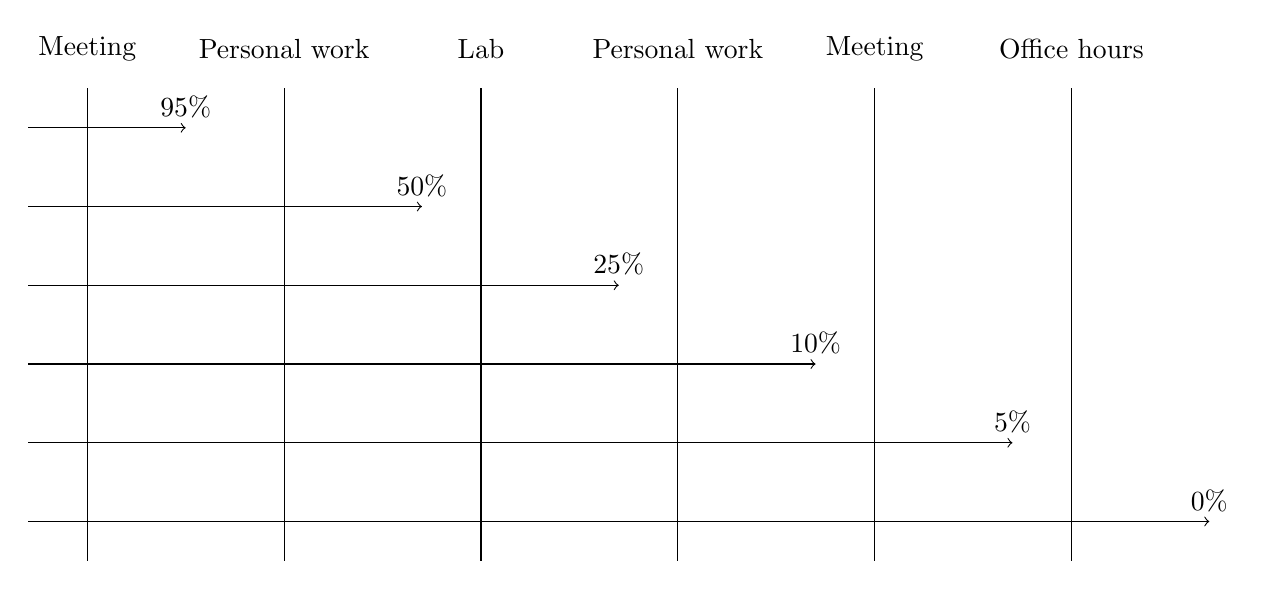
\begin{tikzpicture}
            \foreach \i/\label in {2.5/Meeting,
                                   5/Personal work,
                                   7.5/Lab,
                                   10/Personal work,
                                   12.5/Meeting,
                                   15/Office hours}
                {
                    \draw (\i, -5) -- (\i, 1);
                    \node at (\i, 1.5) {\label};
                }

            \draw [->] (1.75, .5) -- node [above, at end] {95\%} (3.75, .5);
            \draw [->] (1.75, -.5) -- node [above, at end] {50\%} (6.75, -.5);
            \draw [->] (1.75, -1.5) -- node [above, at end] {25\%} (9.25, -1.5);
            \draw [->] (1.75, -2.5) -- node [above, at end] {10\%} (11.75, -2.5);
            \draw [->] (1.75, -3.5) -- node [above, at end] {5\%} (14.25, -3.5);
            \draw [->] (1.75, -4.5) -- node [above, at end] {0\%} (16.75, -4.5);
    \end{tikzpicture}
\end{document}

\part{Further Information}


%\bibliographystyle{plain}
%\bibliography{bibtex_example}

\printindex
\cleardoublepage
\end{document}
